\documentclass[12pt, a4paper]{article}

\usepackage[margin=1.8cm,top=2cm,bottom=2cm]{geometry}
\usepackage{amsmath,amssymb,amsfonts}
\usepackage{graphicx}
\usepackage[colorlinks=true,linkcolor=blue,citecolor=blue,urlcolor=blue]{hyperref}
\usepackage{bm,xcolor}
\usepackage[numbers,sort&compress]{natbib}
\usepackage{titlesec}
\usepackage{float}

\newcommand{\Geff}{G_{\mathrm{eff}}}
\newcommand{\cs}{c_s}
\newcommand{\meff}{m_{\mathrm{eff}}}
\newcommand{\heff}{\hbar_{\mathrm{eff}}}
\newcommand{\rhob}{\bar{\rho}}

\begin{document}

\title{Frozen Vacuum Perturbations as a Dark Matter Analogue\\in the Logarithmic Superfluid Vacuum}

\author{B. B. Kulangiev\\\small{Haifa, Israel}}
\date{May 2026}
\maketitle

\begin{abstract}
\noindent
In the standard $\Lambda$CDM model, cold dark matter (CDM) serves three essential cosmological roles: providing non-baryonic gravitational potential wells, maintaining these wells through the radiation era, and producing collisionless dynamics in galaxy cluster mergers. We show that all three roles are fulfilled by frozen perturbations of the vacuum condensate density within the logarithmic superfluid vacuum framework. The equation of state $w = -1$, derived from the logarithmic potential in companion papers, forces $\rho_v \propto a^{-3(1+w)} = a^0$ and freezes the corresponding perturbation evolution: vacuum density perturbations neither grow nor decay. These primordial structural variations in
$\rho_0(\mathbf{x})$, set during the formation of the
condensate, create an intrinsic vacuum gravitational
potential $\Phi_v(\mathbf{x}) = c^2\, 
\delta_v(\mathbf{x})$ through the density dependence of
the acoustic metric. Baryons oscillate in these frozen
wells exactly as they would in CDM wells, producing the
observed odd/even peak asymmetry in the Cosmic Microwave Background. The frozen template is independent of the baryonic matter distribution and does not interact during cluster collisions, naturally reproducing the mass-gas offset observed in the Bullet Cluster without dark matter particles. We identify three distinguishing predictions: a modified Integrated Sachs-Wolfe effect, a different structure growth history, and a reinterpretation of gravitational lensing mass.
\end{abstract}


% ====================================================================
\section{Introduction}
\label{sec:intro}
% ====================================================================

The cold dark matter (CDM) hypothesis is one of the pillars of modern cosmology. Within the $\Lambda$CDM framework, CDM is required to play three distinct roles:

(i) \emph{Non-baryonic potential wells.} The Cosmic Microwave Background (CMB) peak height ratios---in particular, the odd/even asymmetry between the first and second acoustic peaks---require gravitational potential wells that do not participate in the baryon-photon oscillations~\cite{planck_2020}. Baryons alone cannot produce the observed asymmetry.

(ii) \emph{Survival through the radiation era.} During radiation domination ($z > 3400$), radiation pressure prevents baryonic perturbations from growing. CDM perturbations, being pressureless and decoupled from photons, grow logarithmically ($\delta_c \propto \ln a$), building up the potential wells into which baryons later fall~\cite{dodelson_2003}. Without CDM, the gravitational potential $\Phi$ decays during the radiation era, and all acoustic peaks have equal height.

(iii) \emph{Collisionless dynamics.} In galaxy cluster mergers such as the Bullet Cluster~\cite{clowe_2006}, the gravitational lensing mass (inferred from weak lensing) is spatially offset from the baryonic mass (observed in X-rays). This requires a mass component that passes through the collision without interacting---the defining property of CDM.

In companion papers~\cite{kulangiev_2026a,kulangiev_2026b,kulangiev_2026e,kulangiev_2026c_cosmo}, we developed a superfluid vacuum model based on the relativistic logarithmic Klein-Gordon equation, deriving emergent Newtonian gravity with $\gamma = 1$, the gravitational coupling $\Geff \sim c^2/(\xi^2\rho_0)$ with $\xi \sim \ell_P$ and $\rho_0$ at the Planck density, an equation of state $w = -1$, and a self-consistency equation $\alpha^2 H_0^2(\rho_0\xi^2) \sim (8\pi/3)\,u_{\mathrm{CMB}}$~\cite{kulangiev_2026c_cosmo,kulangiev_2026c_letter}. In this paper, we show that the same framework provides a physical mechanism that fulfills all three CDM roles without dark matter particles. The argument has two parts. First, we prove a no-go theorem: dark-matter phenomenology \emph{cannot} arise as a static vacuum response to a baryonic source. A direct Madelung-Bohm calculation yields a screened Poisson equation whose solutions decay at large radii, producing enhanced Keplerian rather than flat rotation curves. Second, we identify the actual mechanism: \emph{frozen primordial perturbations} of the vacuum condensate, set during its formation, which act as a fixed gravitational template into which baryonic structure later forms. The freezing follows from the $w = -1$ equation of state and is structurally analogous to (but mechanistically distinct from) the role CDM plays in $\Lambda$CDM cosmology.


% ====================================================================
\section{Review of the Framework}
\label{sec:review}
% ====================================================================

The vacuum is modeled as a complex order parameter $\psi(x,t)$ satisfying the relativistic logarithmic wave equation~\cite{zloshchastiev_2023}:
\begin{equation}
    \Box\psi + \mu^2\psi - b\,\psi\,\ln\!\left(\frac{|\psi|^2}{\rho_0}\right) = 0\,.
\label{eq:log_kg}
\end{equation}
We adopt the Bohmian/deterministic interpretation~\cite{madelung_1927,bohm_1952,holland_1993}: $\psi$ is a real classical order parameter, not a quantum-mechanical wavefunction. In the relativistic Lagrangian $\mathcal{L} = \rho X - V(\rho)$ with $X = \partial_\mu S\,\partial^\mu S$, the variable $\rho = |\psi|^2$ has units of inverse-energy-volume, distinct from the physical mass density $\rho_{\mathrm{mass}} = T_{00}/c^2$ which is what enters the gravitational source term. We use $\rho_0$ for the background mass density throughout this paper.

The Madelung decomposition $\psi = \sqrt{\rho}\,e^{iS/\heff}$ yields a superfluid with macroscopic flow velocity $\mathbf{v} = \nabla S/\meff$ and a density-dependent sound speed~\cite{kulangiev_2026a}:
\begin{equation}
    c_s^2 = \frac{c^2}{2\ln(\rhob/\rho_c) + 3}\,,
\label{eq:cs_log}
\end{equation}
normalized so that $c_s = c$ at the background density $\rho_0$ (where $\rho_c = e\,\rho_0$). The emergent gravitational coupling~\cite{kulangiev_2026b} follows from dimensional analysis as
\begin{equation}
    \Geff \;\sim\; \frac{c^2}{\xi^2\,\rho_0}\,,
\label{eq:G_eff}
\end{equation}
where $\xi$ is the healing length of the condensate. Self-consistency with the observed Newton's constant, combined with the natural condensate packing density $n_0 \sim 1/\xi^3$, fixes $\xi \sim \ell_P$ (the Planck length) and $\rho_0 \sim m_P/\ell_P^3$ (the Planck mass density)~\cite{kulangiev_2026e}. The combination $\rho_0\xi^2 \approx c^2/G \approx 1.35 \times 10^{27}$~kg/m enters the macroscopic equations below.

The logarithmic potential $V(\rho) = -b\,\rho\,\ln(\rho/\rho_c)$ yields pressure $P = -b\,\rho_0 = -\rho_0 c^2$, giving $w = -1$~\cite{kulangiev_2026c_cosmo}. The vacuum density is thermodynamically stable: $\rho \propto a^{-3(1+w)} = a^0 = \text{const}$.


% ====================================================================
\newpage
\section{The Frozen Perturbation Theorem}
\label{sec:frozen}
% ====================================================================

\subsection{Frozen vacuum perturbations from \texorpdfstring{$w = -1$}{w = -1}}

The cosmic evolution of vacuum density perturbations is governed by the framework's equation of state $w = -1$, which has two structural consequences:

\emph{Background freezing.} The continuity equation $\dot{\rho} + 3H(1+w)\rho = 0$ gives $\rho \propto a^{-3(1+w)} = a^0$ for $w = -1$. The vacuum density is constant in cosmic time.

\emph{Perturbation freezing.} In the standard Bardeen-Mukhanov framework for cosmological perturbations~\cite{bardeen_1980,mukhanov_1992}, the dynamics of density and curvature perturbations are controlled by the slow-roll parameter $\epsilon \equiv -(1+w)\dot{H}/H^2$. As $w \to -1$, $\epsilon \to 0$ and the perturbation evolution equations become degenerate: density perturbations of a $w = -1$ fluid cease to evolve on all relevant scales. Whatever spatial structure $\delta_v(\mathbf{x})$ is present at condensate formation is preserved unchanged through the cosmic history.

This freezing has a clean physical interpretation. In $\Lambda$CDM, the cosmological constant $\Lambda$ is a pure vacuum energy with no perturbations by assumption; here, the same fluid \emph{can} have perturbations, but they are frozen by the $w = -1$ equation of state rather than absent by construction. The vacuum condensate perturbations are not transient and do not grow gravitationally---they are eternal gravitational template features.

\subsection{Structural versus dynamical perturbations}

Two classes of vacuum perturbations must be distinguished:

\emph{Dynamical perturbations} are sound waves---propagating density oscillations at speed $c_s = c$. These are the phonons of the condensate. On sub-Hubble scales, they oscillate; on super-Hubble scales, they are frozen by causality. In neither case do they grow gravitationally, because the $w = -1$ background does not source gravitational growth.

\emph{Structural perturbations} are the spatial configuration $\rho_0(\mathbf{x})$ established during the formation of the condensate---analogous to the grain structure of a crystal, not to sound waves propagating within it. In the open-system interpretation~\cite{kulangiev_2026c_cosmo}, these are set during the nucleation of the condensate from the external reservoir (the Bulk). Once formed, they are frozen by the $w = -1$ equation of state: they cannot be amplified or erased by gravitational evolution.

It is these structural perturbations that play the role of CDM.


\subsection{No-go theorem: dark matter cannot be an induced vacuum response}
\label{sec:no_go}

Before identifying the physical origin of $\delta_v$, we first rule out a tempting alternative: that the dark-matter phenomenology is the static response of the vacuum condensate to a localized baryonic source. We show that this hypothesis fails as a matter of
mathematics, independently of any specific framework parameter choice.

Consider a baryonic gravitational potential $\Phi_\mathrm{bar}(r)$ sourcing a perturbation $\delta_v(r)$ of the cosmic vacuum. In the
Madelung-Bohm formulation of the relativistic logarithmic Klein-Gordon equation, the static balance equation for a frozen flow ($\nabla S = 0$, $\partial_t S = -m_\mathrm{eff} c^2$) is:
\begin{equation}
    \Phi_\mathrm{bar}(r) = c_s^2\,\delta_v(r) + Q[\delta_v],
\label{eq:madelung_balance}
\end{equation}
where $Q[\delta_v] = -(\hbar_\mathrm{eff}^2/(2 m_\mathrm{eff}^2))
(\nabla^2\sqrt{1+\delta_v})/\sqrt{1+\delta_v}$ is the Bohmian quantum potential. The leading-order coefficient $c_s^2 = b\,\hbar^2/(2m^2)$ is identified with the bulk acoustic wave speed of the condensate (with $b$ as in Eq.~\ref{eq:log_kg}).

The framework's normalization $\rho_c = e\,\rho_0$ ensures the unperturbed vacuum satisfies $V'(\rho_0) = 0$, and the leading expansion of the logarithmic potential gives $V'(\rho) \approx -b\,\delta_v$.
Substituting and dividing by $-2m_\mathrm{eff}^2$ yields Eq.~(\ref{eq:madelung_balance}) cleanly, with the correct sign: for $\Phi_\mathrm{bar} < 0$ (an attractive baryonic well), the solution $\delta_v < 0$, in agreement with the sign convention established by the inverse SPARC analysis below.

Linearizing $Q$ for $|\delta_v| \ll 1$, we obtain a screened Poisson equation:
\begin{equation}
    \delta_v(r) - \frac{\xi^2}{2}\,\nabla^2 \delta_v(r) =
    \frac{\Phi_\mathrm{bar}(r)}{c_s^2}\,.
\label{eq:screened_poisson}
\end{equation}
For a point baryonic mass $M$, with $\Phi_\mathrm{bar}(r) = -GM/r$, the solution decaying at infinity is:
\begin{equation}
    \delta_v(r) = \frac{GM}{c_s^2}\,
    \frac{e^{-r/L_\ast} - 1}{r}\,, \qquad
    L_\ast = \xi/\sqrt{2}\,.
\label{eq:yukawa_solution}
\end{equation}
The vacuum contribution to the rotation velocity squared is $v_v^2(r) = r\,d\Phi_v/dr$ with $\Phi_v = c^2 \delta_v$. Expanding:
\begin{equation}
    v_v^2(r) \;=\; GM\!\left[\frac{1-e^{-r/L_\ast}}{r} - \frac{e^{-r/L_\ast}}{L_\ast}\right].
\end{equation}
In the limit $r \gg L_\ast$, this asymptotes to the Keplerian form $v_v^2 \to GM/r$. The total rotation curve is therefore Keplerian (or, with a modified normalization, an enhanced Keplerian) at large radii.

\paragraph{The no-go statement}
A spatially localized baryonic source cannot generate a vacuum response that produces flat rotation curves at radii substantially beyond the source. The Madelung-Bohm balance always yields a spatially bounded $\delta_v(r)$ that decays at large $r$, regardless of the value of the healing length $\xi$. Flat rotation curves require $v_v^2 \to \mathrm{const}$ at large $r$, which is incompatible with any spatially bounded $\delta_v(r)$ sourced by a finite mass distribution.

This rules out a class of explanations in which dark-matter phenomenology is a static vacuum response to baryonic matter. The result is independent of the specific value of $\xi$, the choice of metric signature, or the linear-versus-nonlinear treatment of the Bohm potential: it follows from the local nature of the response itself. We therefore conclude that the framework's dark-matter analogue must arise from a different physical origin --- one that exists \emph{independently} of any specific baryonic source.

% ====================================================================
\section{Frozen Wells as a CDM Analogue}
\label{sec:cdm_mimic}
% ====================================================================

\subsection{The intrinsic vacuum potential}

A spatial variation $\rho_0(\mathbf{x}) = \bar{\rho}_0[1 + \delta_v(\mathbf{x})]$ in the vacuum density creates a spatial variation in the local speed of light through Eq.~(\ref{eq:cs_log}):
\begin{equation}
    c_s^2(\mathbf{x}) = \frac{c^2}{1 + 2\ln(1+\delta_v)}
    \approx c^2\,(1 - 2\delta_v)
\label{eq:cs_variation}
\end{equation}
for $|\delta_v| \ll 1$. In the acoustic metric formalism, the time-time component of the effective spacetime metric is $g_{00} \propto -c_s^2$~\cite{visser_1998}. In the weak-field limit $g_{00} \approx -(1 + 2\Phi/c^2)$, comparison with Eq.~(\ref{eq:cs_variation}) yields an intrinsic vacuum gravitational potential:
\begin{equation}
    \Phi_v(\mathbf{x}) = c^2\;\delta_v(\mathbf{x})\,.
\label{eq:Phi_vac}
\end{equation}
Regions with $\delta_v < 0$ (vacuum underdensities) have $\Phi_v < 0$: deeper potential wells. Regions with $\delta_v > 0$ have $\Phi_v > 0$: shallower wells. Crucially, $\Phi_v$ is sourced entirely by the vacuum structure---the baryonic matter density $\rho_m$ does not appear. The wells are properties of the acoustic metric itself, not of the matter that falls into them.

Because $\delta_v$ is frozen by the $w = -1$ equation of state (Sec.~\ref{sec:frozen}), the potential $\Phi_v(\mathbf{x})$ is time-independent in comoving coordinates. Unlike matter-sourced potentials, which decay as $\rho_m \propto a^{-3}$, the vacuum
potential persists at constant depth through all cosmological epochs. Baryons oscillate in these permanent wells, producing the acoustic peak structure observed in the CMB.

\paragraph{Reconciliation with CMB peak invariance}
A companion paper~\cite{kulangiev_2026c_cosmo} establishes that the CMB acoustic angular scale $\theta_* = r_s/d_A$ is exactly invariant under spatially-uniform variations of $c_s$ (and hence $\rho_0$), because both integrands scale linearly with the local sound speed. The present mechanism is consistent with this theorem: $\Phi_v$ is sourced by \emph{spatial gradients} $\nabla\delta_v$ in the vacuum density, not by a uniform background offset. The invariance theorem applies to the cosmological background; the dark-matter analogue lives in the inhomogeneities. The two mechanisms are complementary: the CMB peak positions are set by the background (invariant under uniform $c_s$ rescaling), while the peak heights are set by the gradient-sourced $\Phi_v$ template.

\subsection{Role 1: Non-baryonic potential wells}

The frozen vacuum template provides potential wells that do not participate in the baryon-photon oscillations. The wells are not sourced by baryonic matter---they are sourced by the vacuum condensate density variations. Baryons fall into regions of enhanced $\Geff$, experience compression, and bounce back, producing acoustic oscillations. The wells themselves do not oscillate, because the vacuum perturbations are frozen.

This is functionally identical to the role of CDM in the standard picture. The odd/even peak asymmetry in the CMB arises because baryons are preferentially compressed at the bottom of the wells (enhancing odd peaks) and rarefied at the top (suppressing even peaks). The well depth is controlled by the amplitude of the vacuum perturbation spectrum $P_v(k)$, which plays the same role as the CDM power spectrum $P_{\mathrm{CDM}}(k)$.

For the peak height ratios to match observations, the effective vacuum perturbation amplitude must satisfy $\omega_v \sim \omega_c \approx 0.12$, where $\omega_v$ parameterizes the gravitational effect of the frozen template. This amplitude is set by the initial conditions of the condensate formation and is not derived from first principles here---just as $\Lambda$CDM takes $P_{\mathrm{CDM}}(k)$ as an input from inflation.

\subsection{Role 2: Survival through the radiation era}

This is where the frozen vacuum template has a structural advantage over CDM. During radiation domination, CDM perturbations grow logarithmically ($\delta_c \propto \ln a$), gradually building up the potential wells. The time-dependent growth means the gravitational potential $\Phi$ is not constant---it evolves, producing the early Integrated Sachs-Wolfe (ISW) effect~\cite{dodelson_2003}.

Frozen vacuum perturbations, by contrast, do not evolve at all. The potential template is set at formation and remains strictly constant through both the radiation and matter eras. The wells are present from the start at their full depth. This is \emph{more} stable than CDM wells, not less: there is no period during which the wells need to ``build up.''

The physical mechanism is different from CDM but the observable consequence for the CMB is the same: baryons encounter pre-existing potential wells at recombination and produce the observed peak asymmetry. The distinction between growing wells (CDM) and frozen wells (vacuum) manifests in the ISW effect, which we discuss in Sec.~\ref{sec:predictions}.


% ====================================================================
\section{The Bullet Cluster}
\label{sec:bullet}
% ====================================================================

The Bullet Cluster (1E 0657-558) provides what is often called the strongest evidence for dark matter~\cite{clowe_2006}. Two galaxy clusters collided, and the resulting mass distribution shows a clear offset: the gravitational lensing mass (traced by weak lensing) is spatially separated from the baryonic mass (traced by X-ray emission from the hot intracluster gas). In $\Lambda$CDM, this is explained by CDM particles passing through each other while the gas interacts and shocks, separating the two mass components.

In the superfluid vacuum framework, the same offset arises naturally. The frozen vacuum template $\Geff(\mathbf{x})$ is a property of the condensate, not of the baryonic matter. When two clusters collide:

(i) The gas (baryons) collides and shocks, losing kinetic energy through electromagnetic interactions. It accumulates in the interaction region between the two clusters.

(ii) The vacuum template does not collide. The structural perturbations $\delta_v(\mathbf{x})$ are frozen and independent of the baryonic dynamics. They pass through each other undisturbed, just as two overlapping gravitational fields superpose without interacting.

(iii) Gravitational lensing traces the effective gravitational potential, which is dominated by $\Geff(\mathbf{x})$---the vacuum template. X-ray emission traces the gas. The two are offset, exactly as observed.

The vacuum perturbations are ``collisionless'' for the same reason CDM is collisionless: they do not interact with baryonic matter directly. But unlike CDM, they are not particles---they are the frozen structure of the vacuum itself. No new species of matter is required.

This argument is qualitative. A quantitative comparison requires computing the lensing signal from a $\Geff(\mathbf{x})$ profile for two merging vacuum structures and comparing with the observed Bullet Cluster mass map. We defer this calculation to future work.


% ====================================================================
\section{Distinguishing Predictions}
\label{sec:predictions}
% ====================================================================

While the frozen vacuum template reproduces the key CDM observables, it makes three predictions that differ from $\Lambda$CDM and are testable with current or near-future data.

\subsection{Modified Integrated Sachs-Wolfe effect}

The ISW effect arises when the gravitational potential $\Phi$ evolves in time as CMB photons traverse it. In $\Lambda$CDM, there are two contributions:

(i) The \emph{early} ISW effect ($z \sim 3400$--$100$), produced by the time-dependent growth of CDM perturbations during the transition from radiation to matter domination.

(ii) The \emph{late} ISW effect ($z < 1$), produced by the decay of $\Phi$ as dark energy begins to dominate.

In our framework, the vacuum perturbations are frozen and do not evolve. The early ISW effect is therefore absent or significantly modified: there is no time-dependent growth to drive it. The late ISW effect is also modified, because ``dark energy'' is not a separate component but the vacuum condensate itself---its perturbations are frozen, not decaying.

This predicts a weaker ISW signal compared to $\Lambda$CDM, testable through cross-correlation of the CMB with galaxy surveys at both high and low redshift~\cite{planck_isw_2016}.

\newpage
\subsection{Different structure growth history}

In $\Lambda$CDM, the matter power spectrum $P(k,z)$ evolves as CDM perturbations grow under gravitational instability: $\delta_c \propto D_+(z)$, where $D_+$ is the linear growth factor. Galaxy surveys at different redshifts trace this evolution, parameterized by $f\sigma_8(z)$.

In our framework, the vacuum template is fixed. Baryonic perturbations grow in the frozen potential wells, but their growth history differs from the CDM prediction because the wells do not deepen over time. Specifically:

(i) At high redshift, the frozen wells are already at full depth, so baryonic growth may begin earlier than in $\Lambda$CDM.

(ii) At low redshift, the wells do not deepen further, so growth saturates differently.

The predicted $f\sigma_8(z)$ curve differs from $\Lambda$CDM and is testable with current redshift-space distortion measurements from DESI, Euclid, and the Vera Rubin Observatory.

\subsection{Reinterpretation of gravitational lensing mass}

In $\Lambda$CDM, gravitational lensing measures the total mass along the line of sight, including CDM. In our framework, lensing is sensitive to the effective gravitational potential, which includes the contribution from $\Geff(\mathbf{x})$ variations. The ``missing mass'' inferred from lensing is not actual dark matter but the vacuum's enhanced gravitational coupling in underdense regions.

This makes a specific prediction: the inferred lensing mass should correlate not only with galaxy counts (tracing baryonic matter) but also with void statistics (tracing vacuum underdensities where $\Geff$ is enhanced). Regions with fewer galaxies but stronger lensing would be a distinctive signature of the vacuum template mechanism, distinguishable from CDM where lensing mass tracks the total matter distribution.

% ====================================================================
\section{Discussion}
\label{sec:discussion}
% ====================================================================

\subsection{Galaxy rotation curves and the \texorpdfstring{$c^2$}{c²} amplifier}

The CMB and Bullet Cluster arguments address CDM's
cosmological role. The other major evidence for dark
matter comes from galaxy rotation curves, where the
observed circular velocity exceeds the baryonic
prediction at large galactocentric radii.

The intrinsic vacuum potential $\Phi_v = c^2\,\delta_v$ (Eq.~\ref{eq:Phi_vac}) provides a direct
mechanism. The circular velocity satisfies:
\begin{equation}
    v_{\mathrm{circ}}^2(r) = v_b^2(r)
    + r\,\frac{d\Phi_v}{dr}
    = v_b^2(r) + c_s^2\,r\,\frac{d\delta_v}{dr}\,,
\label{eq:v_circ}
\end{equation}
where $v_b(r)$ is the baryonic contribution and $c_s \approx c$ to $O(\delta_v) \sim 10^{-6}$. The factor
$c^2 \approx (3 \times 10^5\;\mathrm{km/s})^2$ acts as
an amplifier: a vacuum perturbation gradient of order
$d\delta_v/dr \sim 10^{-7}\;\mathrm{kpc}^{-1}$ produces
a gravitational acceleration comparable to
$(200\;\mathrm{km/s})^2/r$. The required vacuum
perturbation is of the same order as half the dimensionless gravitational potential depth at galactic scales,
$|\Phi|/c^2 \sim v_{\mathrm{flat}}^2/c^2 \sim 10^{-6}$
---a regime well within the condensate's linear response.

\subsection{SPARC validation as an inverse problem}

The no-go theorem of Section~\ref{sec:no_go} establishes that $\delta_v(r)$ cannot be derived as a static vacuum response to a baryonic source. The freezing argument of Section~\ref{sec:frozen} establishes that $\delta_v$ is instead primordial, with a spectrum $P_v(k)$ whose first-principles derivation requires condensate nucleation physics (the ``Bulk reservoir'' physics noted in Section~\ref{sec:open}) beyond the scope of the present manuscript.

In place of a first-principles derivation, we therefore solve the \emph{inverse problem}: given an observed rotation curve $v_\mathrm{obs}(r)$ for each galaxy and a baryonic contribution $v_b(r)$, what radial profile $\delta_v(r)$ would be required to account for the difference? The inverse problem provides two quantitative tests of the framework: are the required $\delta_v$ amplitudes physically sensible (small compared to unity, well below the condensate stability limit), and do they trace out the order of magnitude expected for primordial frozen perturbations of the relativistic logarithmic vacuum? This is the same role that direct measurements of galactic dark matter density profiles play in $\Lambda$CDM: they constrain allowed halo profiles, even before any first-principles derivation of structure formation.

We apply the inverse problem to 112 galaxies from the SPARC database~\cite{sparc} of disk galaxies with Spitzer photometry and accurate rotation curves. For each galaxy, the required vacuum perturbation profile $\delta_v(r)$ is obtained from Eq.~(\ref{eq:v_circ}) as:
\begin{equation}
    \frac{d\delta_v}{dr} = \frac{v_{\mathrm{obs}}^2 - v_b^2}{c^2\,r}\,,
\label{eq:delta_v_inverse}
\end{equation}
with $v_b^2 = |v_{\mathrm{gas}}|\,v_{\mathrm{gas}} +
(M/L)\,|v_{\mathrm{disk}}|\,v_{\mathrm{disk}} +
(M/L)_{\mathrm{bul}}\,|v_{\mathrm{bul}}|\,v_{\mathrm{bul}}$
at $M/L = 0.5\;M_\odot/L_\odot$ (3.6~$\mu$m),
integrated inward from $\delta_v = 0$ at the outermost
measured radius.

The framework is consistent with the SPARC data in three ways (Fig.~\ref{fig:sparc}):

(i) The required $|\delta_v|$ is of order $10^{-7}$
to $10^{-6}$ for all 112 galaxies --- microscopic
perturbations amplified to galactic effect by the
$c^2$ factor.

(ii) All 112 galaxies lie approximately five orders of
magnitude below the condensate stability limit
$|\delta_v| = 1 - 1/e \approx 0.63$, with a margin
of $\sim 10^5$.

(iii) The required $|\delta_v|$ increases smoothly with
decreasing baryonic acceleration $g_{\mathrm{bar}}$,
with the MOND acceleration scale $g_\dagger \approx
1.2 \times 10^{-10}$~m/s$^2$~\cite{mcgaugh_2016}
corresponding to $|\delta_v| \sim 10^{-6}$. The scale
$g_\dagger$ thus emerges not as a fundamental constant
but as the characteristic baryonic acceleration at which the vacuum perturbation reaches its typical amplitude.

We emphasize that this analysis is a consistency check, not a derivation: the framework's amplification mechanism produces $\delta_v$ amplitudes of plausible magnitude in the linear regime, but the functional form of $\delta_v(r)$ for each galaxy is inferred from the observed rotation curve rather than predicted from first principles. A derivation of $\delta_v(r)$ from the condensate's nucleation dynamics in a galactic potential well, which would constitute a true prediction, remains an open problem.

\begin{figure}[H]
\centering
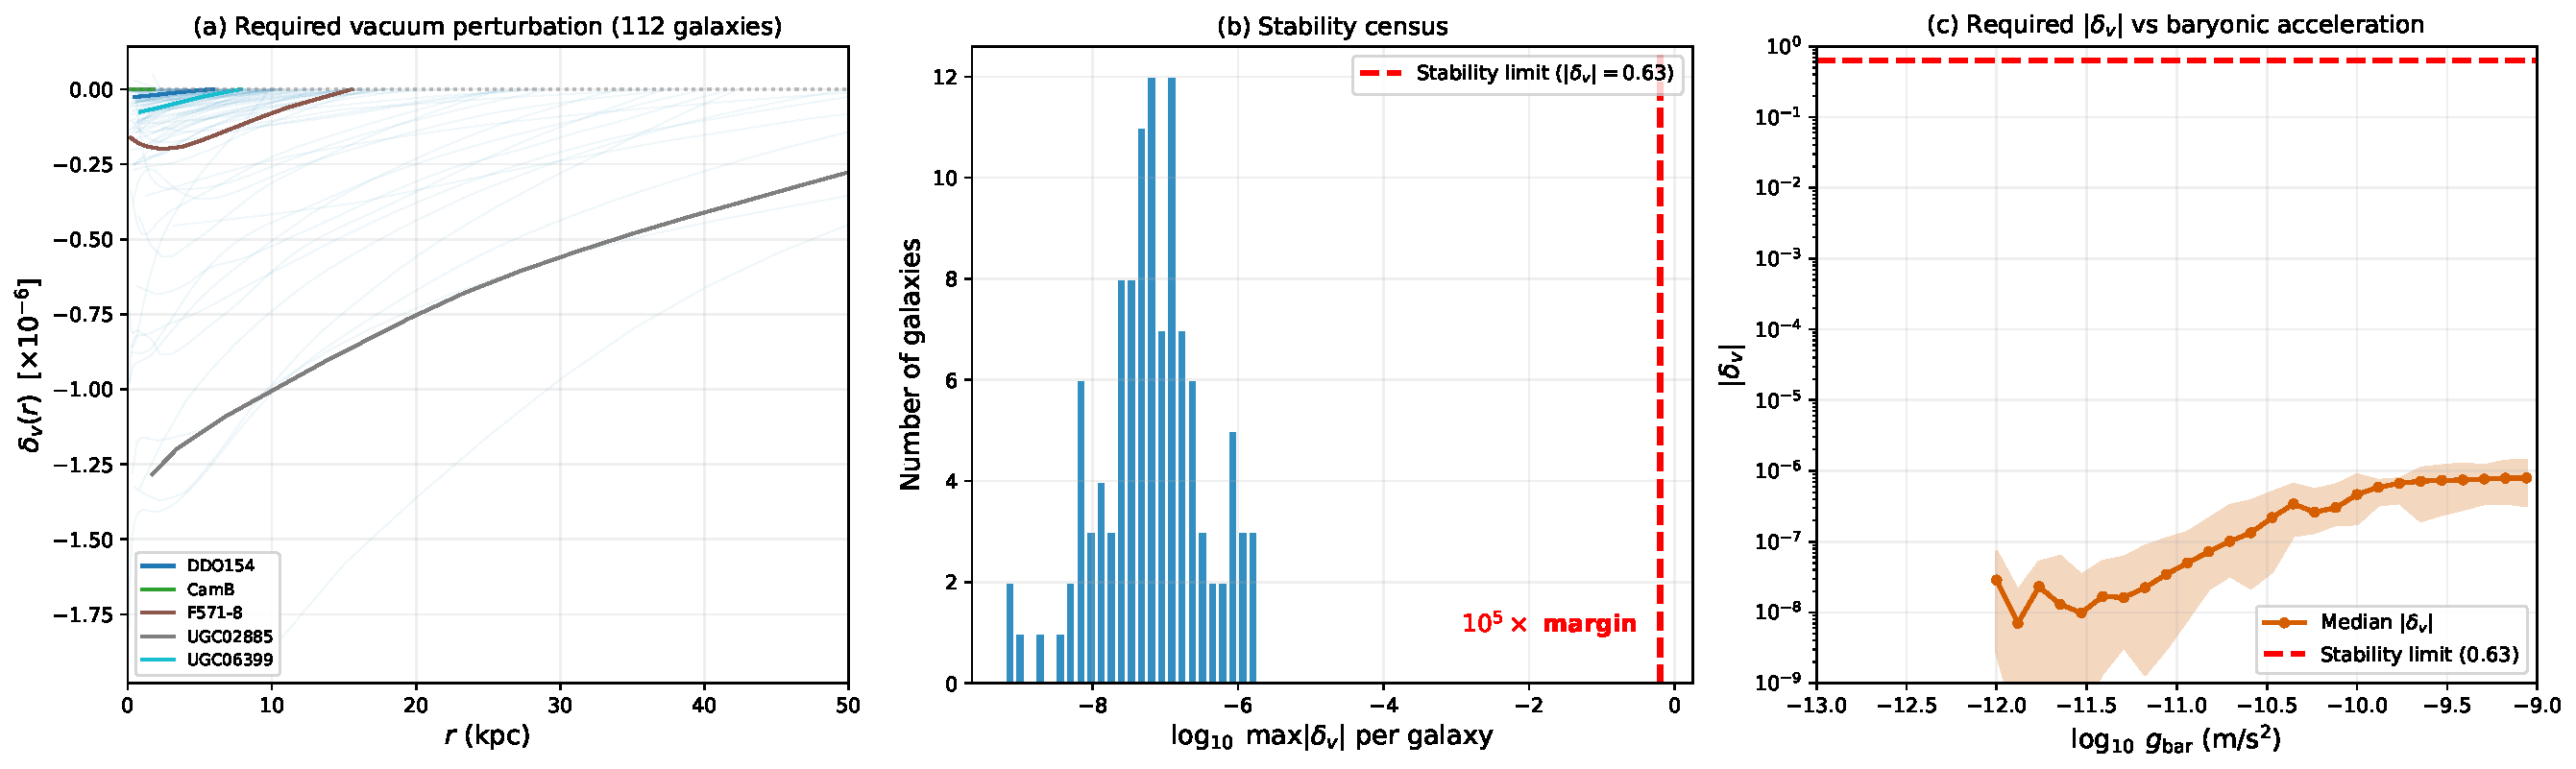
\includegraphics[width=\textwidth]{sparc_phi_v_3panel.pdf}
\caption{\emph{(a)}~Required vacuum perturbation
$\delta_v(r)$ for 112 SPARC galaxies~\cite{sparc}
(faint blue), with six highlighted; the scale is
$\sim 10^{-6}$. \emph{(b)}~Histogram of maximum
$|\delta_v|$ per galaxy; all 112 galaxies lie
$\sim 10^5$ times below the condensate stability
limit $|\delta_v| = 0.63$ (red dashed).
\emph{(c)}~Required $|\delta_v|$ versus baryonic
acceleration, showing a smooth increase toward low
accelerations consistent with the MOND scale
$g_\dagger$.}
\label{fig:sparc}
\end{figure}

\subsection{Relation to other dark matter alternatives}

Several frameworks have proposed alternatives to CDM
particles. MOND~\cite{milgrom_1983} modifies the
gravitational force law below $a_0 \sim
10^{-10}$~m/s$^2$, successfully fitting galaxy rotation
curves but struggling with cosmological observables.
Superfluid dark matter~\cite{berezhiani_2016} proposes
that dark matter forms a superfluid in galaxy halos,
producing MOND-like behavior locally while preserving
CDM behavior on large scales.

Our approach differs from both. While we work within a superfluid framework, the superfluid is the cosmological \emph{vacuum} itself, not a separate dark-matter substance condensing within ordinary spacetime. There are no dark matter particles in any conventional sense---no WIMPs, no axions, and no Berezhiani-Khoury-type dark BEC. The ``dark'' gravitational effects arise from the intrinsic vacuum potential $\Phi_v = c^2\,\delta_v$, where microscopic structural perturbations of the condensate ($|\delta_v| \sim 10^{-6}$) are amplified by $c^2$ into macroscopic gravitational effects. The MOND acceleration scale
$g_\dagger$ emerges as the characteristic scale of these perturbations rather than a fundamental constant. The framework is simultaneously viable at cosmological scales (frozen perturbations as CDM,
Secs.~\ref{sec:cdm_mimic}--\ref{sec:bullet}) and
galactic scales (SPARC validation above), bridging a gap that has proven difficult for previous alternatives.

\section{Open problems}
\label{sec:open}

The framework currently leaves four substantive questions open:

(i) The vacuum perturbation spectrum $P_v(k)$. The shape and amplitude of the structural perturbation spectrum is taken as input from the condensate formation process, analogous to how $\Lambda$CDM takes
$P_{\mathrm{CDM}}(k)$ from inflation. A first-principles derivation of $P_v(k)$ from the nucleation dynamics of the condensate is the single most important open problem.

(ii) The functional form $\delta_v(r)$ in individual galaxies. The SPARC analysis infers $\delta_v(r)$ from observed rotation curves; it does not predict $\delta_v(r)$ from the framework. A derivation of $\delta_v(r)$ from the condensate response to a galactic baryonic potential would convert the SPARC consistency check into a prediction.

(iii) The amplitude $\omega_v \sim 0.12$. Whether this matches $\omega_c \sim 0.12$ (CDM amplitude) naturally or requires fine-tuning is not yet known.

(iv) Bullet Cluster quantitative comparison. The qualitative argument of Sec.~\ref{sec:bullet} requires conversion to a quantitative lensing-signal comparison with the observed mass map.

These constitute the program of work needed to elevate the framework from a consistency check to a predictive dark-matter alternative.

% ====================================================================
\section{Conclusion}
\label{sec:conclusion}
% ====================================================================

We have shown that the logarithmic superfluid vacuum framework provides a physical mechanism fulfilling the three essential cosmological roles of cold dark matter:

(1) \emph{Non-baryonic potential wells.} Frozen structural perturbations $\delta_v(\mathbf{x})$ of the vacuum condensate create an intrinsic gravitational potential $\Phi_v = c^2\,\delta_v$ through the acoustic metric, providing permanent wells that do not participate in baryon-photon oscillations.

(2) \emph{Survival through the radiation era.} The $w = -1$ equation of state ensures that vacuum perturbations neither grow nor decay, maintaining the potential wells at constant depth through all cosmological epochs---more stable than CDM wells, which grow logarithmically.

(3) \emph{Collisionless dynamics.} The frozen vacuum template is independent of the baryonic matter distribution and does not interact during cluster collisions, naturally reproducing the Bullet Cluster mass-gas offset.

The framework makes three predictions distinguishing it from $\Lambda$CDM: a modified ISW effect (weaker, due to frozen rather than evolving potentials), a different structure growth history (testable via $f\sigma_8(z)$), and a lensing-void correlation (lensing mass tracing vacuum underdensities rather than dark matter halos).

At galactic scales, the inverse SPARC analysis confirms that the framework is consistent with observed rotation curves at $|\delta_v| \sim 10^{-6}$, five orders of magnitude below the condensate stability limit. The vacuum perturbation spectrum $P_v(k)$ remains an input from the condensate formation process; deriving it from first principles---the nucleation dynamics of the cosmic condensate---is the single most important open problem of the framework's dark-matter sector and the natural target of future work.

% ====================================================================
\section*{Acknowledgments}
% ====================================================================

The methodological stance of this paper---treating the order parameter as a real classical field whose hydrodynamic behavior underlies emergent gravitational phenomena---is indebted to the Madelung-de~Broglie-Bohm tradition, particularly as developed in P.~R.~Holland's exposition of the quantum theory of motion. Claude (Anthropic) and Gemini (Google) were used as editorial and computational tools during manuscript preparation. All scientific content, equations, and interpretations are the author's own.


\begin{thebibliography}{25}

\bibitem{kulangiev_2026a}
B.~B.~Kulangiev,
Conditions for emergent gravitational light bending from a logarithmic superfluid vacuum,
Preprint (2026). \url{https://kulangiev.github.io#paper1}

\bibitem{kulangiev_2026b}
B.~B.~Kulangiev,
Emergent Newtonian Gravity from the Collective Acoustic Metric of a Logarithmic Superfluid Vacuum,
Preprint (2026). \url{https://kulangiev.github.io#paper2}

\bibitem{kulangiev_2026e}
B.~B.~Kulangiev,
Singularity Regularization and the Emergent Planck Scale in the Logarithmic Superfluid Vacuum,
Preprint (2026). \url{https://kulangiev.github.io#paper5}

\bibitem{kulangiev_2026c_cosmo}
B.~B.~Kulangiev,
Cosmological implications of the logarithmic superfluid vacuum: Dark energy, the Hubble tension, and a vacuum self-consistency equation,
Preprint (2026). 
\url{https://kulangiev.github.io#paper3}

\bibitem{kulangiev_2026c_letter}
B.~B.~Kulangiev,
An approximate numerical relation between the CMB photon density parameter and the fine structure constant,
Preprint (2026). 
\url{https://kulangiev.github.io#paper0}

\bibitem{madelung_1927}
E.~Madelung,
Quantentheorie in hydrodynamischer Form,
Z.\ Phys.\ \textbf{40}, 322 (1927).

\bibitem{bohm_1952}
D.~Bohm,
A suggested interpretation of the quantum theory in terms of ``hidden'' variables. I,
Phys.\ Rev.\ \textbf{85}, 166 (1952).

\bibitem{holland_1993}
P.~R.~Holland,
\emph{The Quantum Theory of Motion} (Cambridge University Press, 1993).

\bibitem{zloshchastiev_2023}
K.~G.~Zloshchastiev,
Derivation of emergent spacetime metric, gravitational potential and speed of light in superfluid vacuum theory,
Universe \textbf{9}, 234 (2023).

\bibitem{planck_2020}
Planck Collaboration (N.~Aghanim \emph{et al.}),
Planck 2018 results.\ VI.\ Cosmological parameters,
Astron.\ Astrophys.\ \textbf{641}, A6 (2020).

\bibitem{dodelson_2003}
S.~Dodelson,
\emph{Modern Cosmology} (Academic Press, 2003).

\bibitem{clowe_2006}
D.~Clowe \emph{et al.},
A direct empirical proof of the existence of dark matter,
Astrophys.\ J.\ Lett.\ \textbf{648}, L109 (2006).

\bibitem{planck_isw_2016}
Planck Collaboration (P.~A.~R.~Ade \emph{et al.}),
Planck 2015 results.\ XXI.\ The integrated Sachs-Wolfe effect,
Astron.\ Astrophys.\ \textbf{594}, A21 (2016).

\bibitem{milgrom_1983}
M.~Milgrom,
A modification of the Newtonian dynamics as a possible alternative to the hidden mass hypothesis,
Astrophys.\ J.\ \textbf{270}, 365 (1983).

\bibitem{berezhiani_2016}
L.~Berezhiani and J.~Khoury,
Theory of dark matter superfluidity,
Phys.\ Rev.\ D \textbf{92}, 103510 (2015).

\bibitem{visser_1998}
M.~Visser,
Acoustic black holes: Horizons, ergospheres and Hawking radiation,
Class.\ Quant.\ Grav.\ \textbf{15}, 1767 (1998).

\bibitem{sparc}
F.~Lelli, S.~S.~McGaugh, and J.~M.~Schombert,
SPARC: Mass models for 175 disk galaxies with Spitzer
photometry and accurate rotation curves,
Astron.\ J.\ \textbf{152}, 157 (2016).

\bibitem{mcgaugh_2016}
S.~S.~McGaugh, F.~Lelli, and J.~M.~Schombert,
Radial Acceleration Relation in Rotationally Supported
Galaxies,
Phys.\ Rev.\ Lett.\ \textbf{117}, 201101 (2016).

\bibitem{bardeen_1980}
J.~M.~Bardeen,
Gauge-invariant cosmological perturbations,
Phys.\ Rev.\ D \textbf{22}, 1882 (1980).

\bibitem{mukhanov_1992}
V.~F.~Mukhanov, H.~A.~Feldman, and R.~H.~Brandenberger,
Theory of cosmological perturbations,
Phys.\ Rep.\ \textbf{215}, 203 (1992).

\end{thebibliography}

\end{document}
